\section{Обзор используемых инструментов}
\label{sec:Chapter2} \index{Chapter2}
\subsection{Языковая модель}
Языковые модели в машинном обучении играют ключевую роль в обработке и понимании естественного языка. \textit{Языковая модель} — это математическая модель, применяемая для расчета вероятности последовательности слов или фраз в естественном языке, обозначаемой как 
$$P(w_1, w_2, ..., w_n)$$
где \(w_1, w_2,..., w_n\) представляют собой токены, обычно слова или n-граммы. Вместо вычисления общей вероятности текста, часто используются модели для оценки условной вероятности 
$$P(w_n| w_1, w_2, ..., w_{n-1})$$
Эти методы являются взаимозаменяемыми, так как полная вероятность может быть выражена через условные вероятности следующим образом:
$$
P(w_1, w_2, ..., w_n) = P(w_1) \cdot P(w_2|w_1) \cdot P(w_3|w_1, w_2) \cdot ... \cdot P(w_n | w_1, w_2, ..., w_{n-1})
$$
Языковые модели лежат в основе множества задач в области обработки естественного языка, включая машинный перевод, автоматическое заполнение, классификацию текстов и другие.

Существуют различные виды языковых моделей, в том числе статистические, такие как скрытые марковские модели (HMM \cite{hmm}), и основанные на нейронных сетях, например, рекуррентные нейронные сети (RNN \cite{Das2023}) и трансформеры.

Статистические модели оценивают вероятность слов на основе их последовательности, что позволяет использовать их для предсказания следующего слова или классификации текста по тематике. Однако они ограничены в понимании контекста слов, что затрудняет их использование для генерации текста.

Нейросетевые языковые модели обучаются на больших объемах данных и могут более точно предсказывать вероятность токенов, что делает их более эффективными для генерации текста, анализа тональности и других задач обработки естественного языка.

В целом, языковые модели являются ключевым инструментом в анализе и обработке естественного языка, находя важное применение в областях, таких как компьютерная лингвистика, машинное обучение и искусственный интеллект. В данной работе, в качестве токенов будут использоваться числа из последовательности ECFP, которые представляют собой молекулярные отпечатки, позволяющие уникально идентифицировать молекулярные структуры.

В контексте машинного обучения, языковая модель представляет собой алгоритм, способный предсказывать следующий элемент в последовательности данных, основываясь на предыдущих элементах. Для текстовых данных, таких как предложения или отпечатки молекул, это означает возможность предсказывать следующее слово или символ. Модель обучается на большом объеме текстовых данных, анализируя контекст и улавливая зависимости между словами. 


\subsection{Модель RoBERTa}

\subsubsection{BPE токенизация} % Roberta
Токенизация - это процесс преобразования текстовых данных в числовой формат, с которым работают методы машинного обучения. Простейший пример токенизации - это разбить текст на части и закодировать каждую часть. Например, можно разбить текст на слова или символы и каждому уникальному слову или символу присвоить свой номер. Однако у этих подходов есть свои недостатки. При кодировании отдельных символов модели будут работать на уровне символов и будет очень сложно восстановить смысл текста по отдельным символам. Со словами возникает проблема в том, что слово может иметь много различных форм, и чтобы учесть все, нужен будет слишком большой словарь, что отрицательно скажется на производительности.

Эффективным решением данной проблемы является Byte Pair Encoding (BPE) \cite{sennrich-etal-2016-neural} токенизация. Принцип работы этого алгоритма следующий: сначала текст кодируется на уровне символов. Затем итеративно выполняются следующие шаги: \begin{itemize} 
\item Выбирается наиболее часто встречающаяся пара токенов
\item Эта пара объединяется в новый токен, и все вхождения этой пары в тексте заменяются на новый токен
\end{itemize}
Процесс повторяется до тех пор, пока размер словаря не достигнет заранее установленного предела. Такой токенизатор обучается на большом корпусе текстов и затем используется для токенизации данных на входе и выходе моделей в процессе их обучения и применения.


\subsubsection{Общая архитектура} % Roberta

\textbf{RoBERTa} (Robustly Optimized BERT Pretraining Approach) \cite{liu2019roberta} представляет собой модель, основанную на архитектуре BERT (Bidirectional Encoder Representations from Transformers) \cite{devlin2019bert}, разработанную в Facebook. Эта модель использует трансформеры для обработки последовательностей входных данных и генерации представлений слов в предложении, учитывая контекст.

\newline
RoBERTa сохраняет основную архитектуру BERT, которая является архитектурой трансформера с механизмом внимания. Математически описать это можно следующим образом:
\begin{equation}
\text{Attention}(Q, K, V) = \text{softmax}\left(\frac{QK^T}{\sqrt{d_k}}\right)V
\end{equation}
где \( Q, K, V \) обозначают матрицы запросов, ключей и значений соответственно, а \( d_k \) — размерность матрицы ключей.
\newline Основная идея BERT заключается в предварительном обучении глубоких двунаправленных представлений от неаннотированного текста, одновременно учитывая контекст слева и справа. Кроме этого, в отличие от оригинальной архитектуры трансформера, которая включает в себя энкодеры и декодеры, BERT использует только энкодеры, что делает его идеальным для задач понимания языка. Однако, в RoBERTa были внесены изменения в процесс предварительного обучения и ключевые гиперпараметры.

\newline
\textbf{Особенности RoBERTa:}
\begin{itemize}
\item RoBERTa не использует задачу Next Sentence Prediction при обучении, что улучшает или по крайней мере не ухудшает производительность на задачах нижнего уровня.
\item Более длительное обучение с большими размерами батчей, что позволяет модели лучше обобщать и достигатьл лучшей точности.
\item Динамическое маскирование: В отличие от BERT, где маскирование выполняется один раз во время предварительной обработки данных, RoBERTa использует динамическую маскирование, что позволяет модели изучать более устойчивые представления.
\item Обучение на большем объеме данных: RoBERTa была обучена на наборе данных объемом 160 ГБ, что в десять раз больше, чем набор данных, использованный для обучения BERT.
\end{itemize}

\newline Схожие модели: CamemBERT и XLM-RoBERTa являются примерами моделей, основанных на RoBERTa, которые, также как и в данной работе, были адаптированы для работы с различными языками.

\newline RoBERTa представляет собой значительное улучшение архитектуры BERT, обеспечивающее более эффективное предварительное обучение и лучшую производительность на широком спектре задач обработки естественного языка.

\subsubsection{Модель RobertaForMaskedLM} % Roberta

RobertaForMaskedLM \cite{roberta_huggingface} — это вариация модели RoBERTa, предназначенная специально для задачи Masked Language Modeling (MLM). Она отличается от стандартной модели RoBERTa тем, что включает в себя дополнительный слой RobertaLMHead, который используется для предсказания вероятности появления слова на месте маски.

% Отличия RobertaForMaskedLM от обычной модели RoBERTa:

% Специализированность: RobertaForMaskedLM оптимизирована для задач MLM, где необходимо предсказать слово, скрытое маской, на основе контекста.
% Структура: В модели RobertaForMaskedLM последний слой предназначен для предсказания маскированных токенов, в то время как стандартная модель RoBERTa может использоваться для различных задач NLP.
% RobertaLMHead — это последний слой в модели RobertaForMaskedLM, который отвечает за предсказание токенов. Этот слой принимает выходные данные из предыдущих слоёв трансформера и применяет линейное преобразование для получения распределения вероятностей по всему словарю.

\newline Принцип работы RobertaForMaskedLM представлен на рисунке \ref{fig:RoBERTaForMaskedLM}. RobertaLMHead получает векторы скрытых состояний от предыдущих слоёв трансформера. Скрытые состояния проходят через линейный слой, который преобразует их в векторы, размерность которых соответствует размеру словаря. Далее применяется функция softmax для получения распределения вероятностей по словарю (здесь модель предсказывает вероятность каждого слова оказаться на месте маскированного токена). 

\begin{figure}[!h]
    \centering
    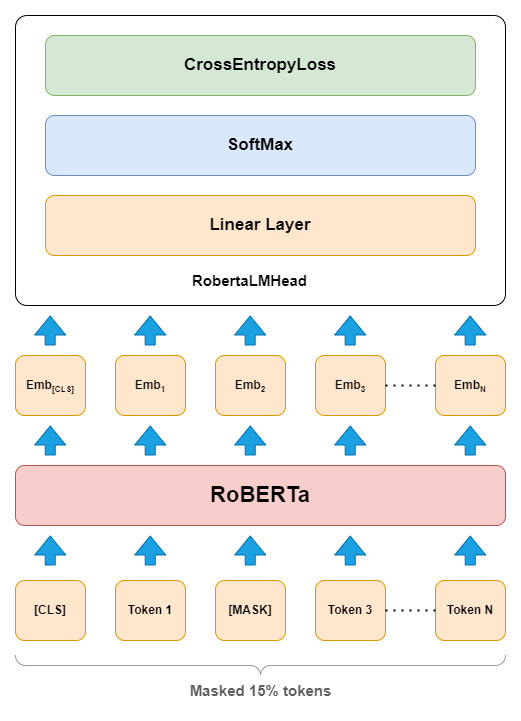
\includegraphics[width = 0.5 \textwidth ]{Bachelor-Thesis-Template/images/robertaMLM.png}
    \caption{\small Принцип работы RoBERTaForMaskedLM.}
    \label{fig:RoBERTaForMaskedLM}
\end{figure}


\newline В дополнительном слое RobertaLMHead используется функция потерь CrossEntropyLoss для вычисления ошибки между предсказанными моделью вероятностями и истинными метками. Это стандартный подход при обучении моделей MLM, таких как RoBERTa. 

Функция CrossEntropyLoss вычисляет, насколько предсказания модели отличаются от фактических меток: 
\begin{equation}
\text{CrossEntropyLoss}(y, \hat{y}) = -\sum_{i} y_{i} \log(\hat{y}_{i})
\end{equation}
где y — истинные метки, а $\hat{y}$ — предсказанные вероятности модели, а суммирование происходит по всем классам (словам в словаре). Функция потерь штрафует модель больше, если предсказанная вероятность для истинного класса низкая, и наоборот, меньше штрафует, если вероятность высокая. Это побуждает модель улучшать свои предсказания с каждой итерацией обучения.

\newline Важно отметить, что веса из слоя встраивания (embedding layer), который преобразует входные токены в векторы, используются повторно для линейного преобразования в RobertaLMHead, что позволяет уменьшить общее количество параметров модели и улучшить её обобщающую способность. Это также известно как “weight tying” в контексте языковых моделей.

\newline В контексте MLM это означает, что модель учится предсказывать вероятность каждого слова в словаре для маскированного токена, и функция потерь оценивает, насколько хорошо модель справляется с этой задачей.

\subsection{ECFP}

\subsubsection{Определение}
\textbf{Extended-Connectivity Fingerprints} - это тип молекулярных отпечатков, специально предназначенных для выявления молекулярных особенностей, связанных с молекулярной активностью. Они являются одними из самых популярных инструментов поиска сходства при разработке лекарств и эффективно используются в самых разных областях применения.

\subsubsection{Алгоритм генерации}
\begin{enumerate}
\item \textbf{Инициализация}: Каждому атому в молекуле присваивается уникальный целочисленный идентификатор, который генерируется путем хеширования комбинации свойств атома.
\item \textbf{Обновление}: На каждом этапе итерации алгоритма ECFP, идентификаторы атомов обновляются путем сбора информации от соседних атомов и применения хеш-функции для создания нового уникального идентификатора.
\item \textbf{Дедупликация}: Удаляются дублирующиеся особенности из сгенерированного списка особенностей, чтобы каждая уникальная подструктура была представлена однократно.
\newline
\newline Эти шаги повторяются для всех атомов в молекуле, позволяя сформировать массив уникальных числовых идентификаторов, которые представляют различные подструктуры молекулы. После завершения всего процесса каждый атом будет иметь идентификатор, который будет содержать субструктурную информацию со всех частей молекулы. Полученный массив чисел может быть использован для анализа молекулярных структур и моделирования структуры. 
\end{enumerate}


\subsubsection{Использование в языковой модели}
Языковые модели могут быть полезны для работы с последовательностями ECFP (Extended Connectivity Fingerprints), которые являются числовым представлением молекулярных структур. Использование языковых моделей в этом контексте может помочь в предсказании эмбеддингов молекул, что, в свою очередь, может облегчить решение различных задач, связанных с молекулярным моделированием и анализом.

Языковые модели (особенно те, что основаны на нейронных сетях, такие как BERT или Graph Neural Networks) могут изучать сложные зависимости и паттерны в данных. Они способны обрабатывать последовательности токенов и предсказывать вероятности следующих токенов и/или их векторные представления. В случае ECFP, которые кодируют информацию о химической структуре молекул, языковые модели могут использоваться для генерации представлений, которые отражают молекулярные свойства и потенциальные биологические активности.

Таким образом, подавая ECFP в качестве входных данных для языковой модели, можно обучить модель предсказывать эмбеддинги, которые могут быть использованы для различных приложений, таких как поиск похожих молекул, предсказание фармакологических свойств или оптимизация молекулярных структур для улучшения желаемых характеристик.
Важно отметить, что успех такого подхода зависит от качества и количества обучающих данных, а также от способности модели обрабатывать специфику молекулярных фингерпринтов. Это может потребовать тонкой настройки и адаптации существующих языковых моделей под конкретные задачи в области химии и молекулярной биологии.


\subsubsection{Применение к BPE токенизатору}
В рамках исследования был предложен подход к применению алгоритма Byte Pair Encoding (BPE) \cite{sennrich-etal-2016-neural} для токенизации отпечатков ECFP, представленных в виде массива чисел. Достаточно представить имеющиеся отпечатки как строку, где словами будут являться числа из массива молекулы.

\textbf{Более формально}:
Зафиксируем молекулу. Пусть \( E = \{e_1, e_2, \ldots, e_n\} \) будет её массивом ECFP, где каждый элемент \( e_i \) представляет собой целочисленное значение, полученное в результате хеширования молекулярных подструктур. Этот массив преобразуется в строку \( S \), где каждое число \( e_i \) представлено как отдельное слово (слова разделены пробелом):
$$ S = "e_1\ e_2\ \ldots\ e_n" $$

Далее, к строке \( S \) применяется алгоритм BPE, который итеративно заменяет наиболее часто встречающиеся пары чисел на новые токены, уменьшая тем самым размер словаря и обеспечивая компактное представление входных данных для модели.

Экспериментальные результаты показали, что предложенный метод токенизации ECFP с использованием BPE позволяет трансформерам эффективно обрабатывать молекулярные данные, сохраняя при этом значимую информацию о структуре и свойствах молекул.

\subsubsection{Сравнение с SMILES}
В отличие от SMILES, которые представляют линейную последовательность символов для описания молекул, ECFP генерируют векторы, которые кодируют более сложную информацию о молекуле, включая её топологическое расположение и химические свойства. Это делает ECFP особенно полезными для задач, где требуется улавливать сложные молекулярные взаимодействия и свойства, таких как предсказание биологической активности или свойств связывания.

\subsection{Графовая модель}
Графовые нейронные сети (GNN) - это тип искусственных нейронных сетей, предназначенный для работы с данными, структурированными в виде графов. Графы — это математические конструкции, которые используются для представления объектов и их связей, где узлы — объекты, а ребра — связи между ними.

В отличие от обычных нейронных сетей, которые созданы для ввода в виде сетки, GNN работают непосредственно с графами. Они способны изучать представления на уровне узлов и графов, которые полезны для широкого круга задач. Например, GNN можно использовать для задач классификации узлов, целью которых является присвоение метки каждому узлу в графе на основе его характеристик и характеристик его соседей. GNN также можно использовать для задач классификации графов, целью которых является прогнозирование свойств всего графа на основе его структуры и особенностей.

В контексте молекулярных структур, графовые нейронные сети могут быть особенно полезны. Молекулы можно представить в виде графов, где атомы являются узлами, а химические связи - ребрами. GNN могут быть использованы для изучения этих молекулярных графов, предсказания их свойств, и даже для генерации новых потенциальных молекул для лекарственного дизайна. Это делает GNN мощным инструментом в области компьютерной химии и биоинформатики.



\subsection{Модель GCN}
Graph Convolutional Network (GCN) \cite{kipf2017semisupervised} - это класс графовых нейронных сетей, который использует операцию свертки в контексте графовых структур данных. Основное отличие слоя GCN от линейного слоя заключается в том, что GCN учитывает структуру графа и связи между узлами при обновлении своих весов.

В традиционных нейронных сетях линейные слои применяют линейное преобразование к входным данным. Это преобразование преобразует входные характеристики $x$ в скрытые векторы $h$ с использованием матрицы весов $\mathbf{W}$. Если на время не учитывать смещения, это можно выразить как: 
$$h = \mathbf{W}x$$

С данными графа добавляется дополнительный слой сложности через связи между узлами. Эти связи важны, потому что, как правило, в сетях предполагается, что похожие узлы скорее будут связаны друг с другом, чем непохожие, явление, известное как гомофилия сети.

Мы можем обогатить наше представление узла, объединив его характеристики с характеристиками его соседей. Эта операция называется сверткой или агрегацией по соседству. Давайте обозначим окрестность узла i, включая сам узел, как $N_{i}$
$$h_{i} = \sum_{j \in N_{i}}\mathbf{W}x_{j}$$

Наши сверточные нейронные сети (CNN) отличаются тем, что у нас есть уникальная матрица весов $\mathbf{W}$, которая используется всеми узлами. Однако мы сталкиваемся с проблемой: количество соседей у узлов не фиксировано, в отличие от пикселей.

Чтобы значения для всех узлов были сопоставимы и находились в одном диапазоне, мы можем нормализовать результат, учитывая степень узлов, где под степенью понимается количество связей узла.
$$h_{i} = \frac{1}{deg(i)} \sum_{j \in N_{i}}\mathbf{W}x_{j}$$

Введенный Кипфом и др. (2016), у слоя графовой свертки есть еще одно улучшение.
Авторы заметили, что признаки от узлов с большим количеством соседей распространяются гораздо легче, чем от более изолированных узлов. Чтобы компенсировать этот эффект, они предложили присваивать большие веса признакам от узлов с меньшим количеством соседей, тем самым балансируя влияние по всем узлам. Эта операция записывается как
\begin{equation}
h_{i} = \sum_{j \in N_{i}} \frac{1}{\sqrt{deg(i)deg(j)}} \mathbf{W}x_{j}
\end{equation}

Существуют различные модификации слоя GCN, которые вносят улучшения или изменения в базовую модель GCN для улучшения производительности или адаптации к конкретным типам задач. Например, некоторые модификации могут включать в себя различные стратегии агрегации информации из соседних узлов или использование различных типов весовых матриц.

В отношении известных моделей, использующих GCN, можно отметить, что GCN является основой для многих других архитектур графовых нейронных сетей. Например, Graph Attention Networks (GAT) \cite{veličković2018graph} и Message Passing Neural Networks (MPNN) \cite{maskey2022generalization} являются двумя известными архитектурами, которые используют GCN в качестве основы.


\subsection{Модель MolCLR}
Molecular Contrastive Learning of Representations (MolCLR) \cite{molclr} была представлена в работе Юянга Ванга и его коллег в 2022 году. Основная архитектура модели представлена на рисунке \ref{fig:MolCLR}.

MolCLR использует подход контрастного обучения для обучения представлений молекул на больших неразмеченных наборах данных (порядка 10 миллионов молекул). Этот подход значительно улучшает производительность моделей графовых нейронных сетей на различных задачах прогнозирования свойств молекул.

В основе MolCLR лежит идея, что молекулы, которые имеют схожую структуру или свойства, должны иметь близкие представления в пространстве признаков. Для достижения этого MolCLR использует Contrastive Loss: модель обучается минимизировать расстояние между позитивными парами (то есть молекулами, которые считаются схожими) и максимизировать расстояние между негативными парами (то есть молекулами, которые считаются различными).

В модели MolCLR используются слои GCN \cite{kipf2017semisupervised} или GIN (Graph Isomorphism Network \cite{kim2020understanding}) для кодирования графов молекул. Эти слои графовых нейронных сетей позволяют модели эффективно обрабатывать структурную информацию о молекулах и извлекать из нее полезные признаки.

В данном подходе предлагаются три стратегии аугментации графа молекул: маскирование атомов, удаление связей и удаление подграфов. Эти аугментации применяются к графам молекул, чтобы создать “позитивные” пары (то есть пары аугментаций из одной и той же молекулы), которые модель стремится приблизить в пространстве признаков. 

\begin{figure}[!h]
    \centering
    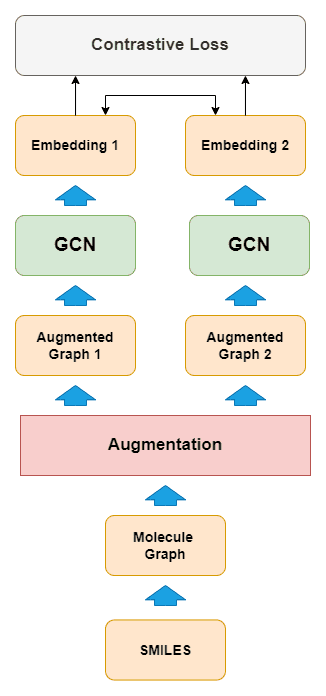
\includegraphics[width = 0.4 \textwidth ]{Bachelor-Thesis-Template/images/molclr/molclr.png}
    \caption{\small Архитектура модели MolCLR.}
    \label{fig:MolCLR}
\end{figure}

После предварительного обучения с использованием контрастного обучения, MolCLR может быть дообучена на конкретной задаче прогнозирования свойств молекул, такой как прогнозирование растворимости или токсичности.

Важно отметить, что благодаря предварительному обучению на больших неразмеченных наборах данных, MolCLR показывает хорошие результаты на различных задачах прогнозирования свойств молекул.

\subsection{Модель Graphormer}
\textbf{Graphormer} \cite{graphormer} — это модель глубокого обучения, разработанная Microsoft Research Asia и основанная на архитектуре Transformer, адаптированная для работы с графами. Основное отличие Graphormer заключается в эффективном кодировании структурной информации графа в модель, что достигается за счет использования специальных методов структурного кодирования. Она показала отличные результаты в различных задачах представления графов, особенно в рамках OGB Large-Scale Challenge.

Graphormer может быть полезен по нескольким причинам:
\begin{enumerate}
    \item Graphormer эффективно кодирует структурную информацию графа, что делает его подходящим для моделирования молекулярных структур.
    \item Данная модель показала отличные результаты на широком диапазоне задач обучения представлению графов.
    \item Graphormer может быть использован для обучения пользовательских моделей для задач моделирования молекул.
    \item Graphormer может покрывать многие популярные варианты GNN в качестве своих специальных случаев.
\end{enumerate}

Для подготовки данных к обучению Graphormer необходимо использовать специальную функцию collate, которая группирует признаки нескольких графов в батчи. Это позволяет эффективно подавать данные в модель. Предобработка включает в себя преобразование данных в формат, совместимый с Graphormer, включая создание объектов DGLGraph и использование стандартного PyTorch Dataloader для подачи данных в модель.

Обучение Graphormer включает в себя стандартные этапы, такие как маскирование части входных данных и предсказание вероятностей для замаскированных элементов. Важно отметить, что модель может неэффективно работать с очень большими графами (более 100 вершин), так как это может привести к переполнению памяти. В таких случаях рекомендуется уменьшить размер батча или использовать более мощные вычислительные ресурсы.



\subsection{Графовое представление молекул}

\begin{enumerate}
    \item  Узлы представляют собой молекулярные атомы. Каждый узел имеет свой уникальный идентификатор (например, атомный номер) и может содержать дополнительные атрибуты (например, химические свойства атома).
    \item Рёбра соединяют узлы и представляют химические связи между атомами. В графовых представлениях молекул обычно используются два типа рёбер:
    \begin{itemize}
        \item \texttt{edge\_index}: Это список пар узлов, которые соединены рёбрами. Например, если у нас есть ребро между атомами 1 и 2, то (1, 2) будет присутствовать в \texttt{edge\_index}. Таким образом, размер этого поля $2*|E|$, где $|E|$ – количество рёбер в графе.
        \item \texttt{edge\_attr}: Это матрица признаков рёбер, таких как тип связи (одинарная, двойная, тройная) или расстояние между атомами.
    \end{itemize}
    \item Атрибуты узлов (\texttt{node\_attr}): Это матрица, состоящая их дополнительных характеристик каждого узла. Например, масса атома, заряд, гибридизация и т. д.
    \item Количество узлов (\texttt{num\_nodes}): Это общее количество атомов в молекуле.
\end{enumerate}
В графовых моделях, таких как MolCLR и Graphormer, на вход графы подаются в формате, который содержит данные поля, поэтому они играют важную роль в обучении подобных моделей.

\subsection{Библиотека RDKit}
\textbf{RDKit} \cite{RDKit} – это библиотека для хемоинформатики и машинного обучения, написанная на C++ и Python. RDKit предоставляет множество функций для работы с молекулами, включая чтение, отображение, запись и многие другие операции.
Есть возможность создавать молекулы из SMILES-кодов, файлов формата MOL и блоков данных MOL, а также поддерживается отображение молекул в виде графических изображений.
 
Пример получения обьекта молекулы из SMILES: 
$$\texttt{rdkit.Chem.MolFromSmiles('Cc1ccccc1')}$$

\subsection{Датасет ChemBL}
\textbf{ChEMBL} \cite{ChemBL} – это база данных биоактивных молекул с лекарственными свойствами. Она объединяет химические, биоактивные и геномные данные для поддержки перевода геномной информации в эффективные новые лекарства.

На основе данных из данного датасета можно получить молекулярные фингерпринты или SMILES и обучить модель машинного обучения для регрессии молекулярных свойств, используя различные алгоритмы, такие как графовые нейронные сети (GNN), регрессию или другие методы. Таккже можно использовать датасет ChEMBL для тестирования полученных моделей, так как он предоставляет информацию о биоактивных молекулах и их свойствах.

\subsection{Оптимизатор AdamW}}
\textbf{AdamW} \cite{adamw} — один из самых эффективных алгоритмов оптимизации для обучения нейронных сетей. Это модификация оптимизационного алгоритма Adam (adaptive moment estimation), который сочетает в себе идеи RMSProp и оптимизатора импульса. Adam использует адаптивную оценку моментов первого и второго порядка.
\begin{itemize}
    \item Основная идея AdamW заключается в добавлении метода декремента весов (weight decay) к Adam.
    \item Декремент весов помогает бороться с переобучением, регуляризуя модель.
    \item AdamW более устойчив к большим значениям весов и улучшает обобщающую способность модели.
\end{itemize}

\subsection{Функции потерь}
\subsubsection{L1-Loss}
Для L1-потерь обычно используется MAE (Mean Absolute Error):
\begin{equation}
L1 = \sum_{i=1}^{N} |y_i - \hat{y}_i|
\end{equation}
где $N$ - количество элементов во входе $y$, $y_i$ - фактическое значение для i-го примера, а $\hat{y}_i$ - предсказанное значение для i-го примера.

\subsubsection{MSE-Loss}
Функция потерь Mean Squared Error (MSE) измеряет среднеквадратичную ошибку (квадрат нормы L2) между каждым элементом входа x и целевым значением y. Она описывается следующим образом:
\begin{equation}
\ell(y, \hat{y}) = \frac{1}{N} \sum_{n=1}^{N} (y_n - \hat{y}_i)^2 
\end{equation}
где $N$ - количество элементов во входе $y$, $y_i$ - фактическое значение для i-го примера, а $\hat{y}_i$ - предсказанное значение для i-го примера.

\subsubsection{CosineSimilarityLoss}
\textbf{Cosine Similarity Loss} используется для измерения сходства между двумя векторами на основе косинусного сходства. Это часто применяется для оценки степени схожести между векторами. Значение косинусного сходства находится в диапазоне от -1 до 1, где 0 указывает на ортогональность, а значения, близкие к 1 по модулю, указывают на большее сходство.
Формула косинусного расстояния:
\begin{equation}
sim(x_1, x_2) = \frac{x_1 * x_2}{max(\lVert x_1 \rVert * \lVert x_2 \rVert, \epsilon)}
\end{equation}

\subsubsection{NTXentLoss}
\textbf{NT-XentLoss} (Normalized Temperature-scaled Cross Entropy Loss) — это функция потерь, используемая в глубоком обучении. Она измеряет косинусное сходство между двумя векторами и использует параметр температуры для балансировки положительных и отрицательных пар. Пусть $sim(u, v)$ обозначает косинусное сходство между векторами u и v. Тогда функция потерь для положительной пары примеров (i, j) выглядит следующим образом:

\begin{equation}
l_{i, j} = -\log\left(\frac{e^{sim(u_i, v_j) / \tau}}{\sum_{k=1}^{N} e^{sim(u_i, v_k) / \tau}}\right)
\end{equation}

где $sim(u_i, v_j)$ - косинусное сходство между векторами $u_i$ и $v_j$, $N$ - общее количество примеров, $\tau$ (температура) - параметр, который регулирует вклад положительных и отрицательных пар.

Эта функция потерь позволяет обучать эмбеддинги так, чтобы они были близки для положительных пар и далеки для отрицательных пар, что полезно для задач, связаных с поиском сходства между векторами, например, в задачах ранжирования или рекомендации.


\newpage
